\documentclass{article}
\usepackage[utf8]{inputenc}
\usepackage[spanish]{babel}
\usepackage{graphicx}
\usepackage{anysize}
\usepackage{fancyhdr} 
\usepackage[export]{adjustbox}
\usepackage{titlesec}
\usepackage{enumitem}
\usepackage{amsmath}
\usepackage{amssymb}
% \usepackage{hyperref}
% \usepackage{float}
% \usepackage{tabu}
\usepackage[table, svgnames, dvipsnames]{xcolor}

% Izquierda, derecha, arriba, abajo
\marginsize{1.5cm}{2cm}{1.2cm}{1cm} 
\renewcommand{\familydefault}{\sfdefault}
\decimalpoint%

\graphicspath{{assets/}{bdd_prac_04.assets/}}

\setlength{\parindent}{0in}
\titleformat*{\section}{\large\bfseries}

\newcommand{\materia}{BDD}
\newcommand{\clave}{2947}
\newcommand{\profesor}{Ing. Rodriguez Campos \textsc{Jorge Alberto}}
\newcommand{\grupo}{1}
\newcommand{\semestre}{2021-1}

\newcommand{\alumno}{Francisco Pablo \textsc{Rodrigo}}

\newcommand{\actividad}{Práctica 04}
\newcommand{\titulo}{Diseño del esquema de fragmentación}

\newcommand{\fechaEntrega}{22 de octubre de 2020}

%%%%%%%%%%%%%%%%%%%% ENCABEZADO %%%%%%%%%%%%%%%%%%%%%%%%%%%%
\pagestyle{fancy}
\fancyhf{}
\renewcommand{\headrulewidth}{0pt}
\fancyhead[R]{% Left header
    \begin{tabular}{l}
        \materia \\ 
        \actividad%
    \end{tabular}
    \,% Space
    \rule[-1.75\baselineskip]{0pt}{0pt}
    % Strut to ensure a 1/4 \baselineskip between image and header rule
    
\includegraphics[height=3\baselineskip,valign=c]{unam}
}
\setlength{\headsep}{0.3in}


\begin{document}
%%%%%%%%%%%%%%%%%%% DATOS PORTADA %%%%%%%%%%%%%%%%%%%%%%%%
\thispagestyle{empty}
\begin{minipage}[t][5cm][t]{0.2\linewidth}
    
\includegraphics[width=2.5cm]{unam.jpg}
    \vspace{10cm}

    
\includegraphics[width=2.5cm]{fiblack}
\end{minipage}
\begin{minipage}[t]{0.7\linewidth}
    \vspace{-2.5cm}
    \LARGE{\textbf{Universidad Nacional Autónoma de México}}\\
    \Large{\textbf{Facultad de Ingeniería}} \\

    \large{\semestre}\\[2cm]

    \large{\textbf{\materia (\clave)}}\\
    \large{\textbf{Gpo: 1}}\\[5mm]
    \large{\textbf{Profesor:} \profesor}\\ [1.5cm]
    \begin{center}
        \LARGE{\textbf{\actividad}}\\
        \LARGE{\textbf{\titulo}}\\
    \end{center}

    \vspace{3.3cm}

    \large{\textbf{Alumno:} \alumno} \\[1.5cm]

    \begin{flushright}
        \fechaEntrega%
    \end{flushright}
\end{minipage}

\newpage
%%%%%%%%%%%%%%%%%%% CONTENIDO %%%%%%%%%%%%%%%%%%%%%%%%

\section*{Introducción}
% TODO:- Hacer introducción en tiempo futuro
En esta práctica se analiza un caso de estudio más completo para aplicar 
los conceptos de fragmentación. A manera de recordatorio se tienen 3 tipos de 
fragmentación: i) fragmentación Horizontal (primaria y derivada); ii) 
fragmentación vertical; iii) fragmentación mixta o híbrida. Así mismo, a la
hora realizar la fragmentación no debemos olvidar que los esquemas locales
deben de cumplir con las tres reglas básicas de la fragmentación: completitud,
reconstrucción y exclusión (no aplica para fragmentación vertical). Por último,
es altamente recomendable realizar todos los esquemas necesarios para facilitar
el proceso de fragmentación (división por tabla, árbol de reconstrucción).
\section*{Objetivos}
Poner en práctica los conceptos de fragmentación y sus diversos tipos a través 
de su implementación en un ambiente distribuido de 2 nodos.

\section*{C1. Esquema de fragmentación (tabla)}
\newcommand{\nomtabla}[1]{F\_RFP\_#1}
\newcounter{numFrags}
\begin{table}[h!]
\def\arraystretch{2}
% \setlength{\tabcolsep}{10pt}
\begin{tabular}{|c|c|c|c|}
\hline
Núm. &
Nombre del fragmento & Expresión del fragmento & 
\parbox[t]{2cm}{Ubicación del\\ fragmento\\ (N1 o N2)} \\ \hline
% fila 1
\stepcounter{numFrags} \arabic{numFrags} &
\nomtabla{SUSCRIPTOR\_1} & 
\begin{minipage}[b]{8.3cm}
    \begin{equation*} 
         = \pi_{\text{suscriptor\_id,num\_tarjeta}}(\text{SUSCRIPTOR})
    \end{equation*}
\end{minipage}  & 
N\_1 \\ \hline
% fila 2
\rowcolor{Gainsboro!60}
 &
\nomtabla{SUSCRIPTOR\_2'} & 
\begin{minipage}[b]{8.3cm}
    \begin{equation*} 
         = \pi_{\substack{\text{suscriptor\_id,nombre, ap\_pat, ap\_mat,}\\ 
         \text{fecha\_inscripcion, pais\_id}}}(\text{SUSCRIPTOR})
    \end{equation*}
\end{minipage}  & 
 \\ \hline
% fila 3
\stepcounter{numFrags} \arabic{numFrags} &
\nomtabla{PAIS\_1} & 
\begin{minipage}[b]{8.3cm}
    \begin{equation*} 
         = \sigma_{\text{reg\_economica=`A'}}(\text{PAIS})
    \end{equation*}
\end{minipage}  & 
N\_1 \\ \hline
% fila 4
\stepcounter{numFrags} \arabic{numFrags} &
\nomtabla{PAIS\_2} & 
\begin{minipage}[b]{8.3cm}
    \begin{equation*} 
         = \sigma_{\text{reg\_economica=`B'}}(\text{PAIS})
    \end{equation*}
\end{minipage}  & 
N\_2 \\ \hline
% fila 5
\stepcounter{numFrags} \arabic{numFrags} &
\nomtabla{SUSCRIPTOR\_2} & 
\begin{minipage}[b]{8.3cm}
    \begin{equation*} 
         = \text{\nomtabla{SUSCRIPTOR\_2'}} \ltimes_{\text{suscriptor\_id}} \text{\nomtabla{PAIS\_1}}
    \end{equation*}
\end{minipage}  & 
N\_1 \\ \hline
% fila 6
\rowcolor{Gainsboro!60}
&
\nomtabla{SUSCRIPTOR\_3'} & 
\begin{minipage}[b]{8.3cm}
    \begin{equation*} 
         = \text{\nomtabla{SUSCRIPTOR\_2'}} \ltimes_{\text{suscriptor\_id}} \text{\nomtabla{PAIS\_2}}
    \end{equation*}
\end{minipage}  & 
 \\ \hline
% fila 7
\stepcounter{numFrags} \arabic{numFrags} &
\nomtabla{SUSCRIPTOR\_3} & 
\begin{minipage}[b]{8.3cm}
    \begin{equation*} 
        % TODO:- Agregar SQL valido
        %  = \sigma_{\text{ap\_paterno[1] between `A' and `M'}}
         = \sigma_{\substack{\text{substr(ap\_paterno,1,1)}\\ \text{between `A' and `M'}}}
         (\text{\nomtabla{SUSCRIPTOR\_4'}})
    \end{equation*}
\end{minipage}  & 
N\_1 \\ \hline
% fila 8
\stepcounter{numFrags} \arabic{numFrags} &
\nomtabla{SUSCRIPTOR\_4} & 
\begin{minipage}[b]{8.3cm}
    \begin{equation*} 
        % TODO:- Agregar SQL valido
        %  = \sigma_{\text{ap\_paterno[1] between `N' and `Z'}}
         = \sigma_{\substack{\text{substr(ap\_paterno,1,1)}\\ \text{between `N' and `Z'}}}
         (\text{\nomtabla{SUSCRIPTOR\_4'}})
    \end{equation*}
\end{minipage}  & 
N\_2 \\ \hline
% fila 9
\stepcounter{numFrags} \arabic{numFrags} &
\nomtabla{ARTICULO\_1} & 
\begin{minipage}[b]{8.3cm}
    \begin{equation*} 
         = \pi_{\text{articulo\_id,pdf}}(\text{ARTICULO})
    \end{equation*}
\end{minipage}  & 
N\_2 \\ \hline
% fila 10
\stepcounter{numFrags} \arabic{numFrags} &
\nomtabla{ARTICULO\_2} & 
\begin{minipage}[b]{8.3cm}
    \begin{equation*} 
         = \pi_{\text{articulo\_id,titulo,resumen,texto}}(\text{ARTICULO})
    \end{equation*}
\end{minipage}  & 
N\_1 \\ \hline
% fila 11
\stepcounter{numFrags} \arabic{numFrags} &
\nomtabla{REVISTA\_1} & 
\begin{minipage}[b]{8.3cm}
    \begin{equation*} 
        % TODO:- Agregar SQL valido
        % = \sigma_{\text{fecha\_publ $\in$ [enero,junio]}}(\text{REVISTA})
        = \sigma_{\text{to\_char(fecha\_publ,`mm') between `01' and `06'}}(\text{REVISTA})
    \end{equation*}
\end{minipage}  & 
N\_1 \\ \hline
% fila 12
\stepcounter{numFrags} \arabic{numFrags} &
\nomtabla{REVISTA\_2} & 
\begin{minipage}[b]{8.3cm}
    \begin{equation*} 
        % TODO:- Agregar SQL valido
        % = \sigma_{\text{fecha\_publ $\in$ [julio,diciembre]}}(\text{REVISTA})
        = \sigma_{\text{to\_char(fecha\_publ,`mm') between `07' and `12'}}(\text{REVISTA})
    \end{equation*}
\end{minipage}  & 
N\_2 \\ \hline
% fila 13
\stepcounter{numFrags} \arabic{numFrags} &
\nomtabla{ARTICULO\_REVISTA\_1} & 
\begin{minipage}[b]{8.3cm}
    \begin{equation*} 
        = \text{ARTICULO\_REVISTA} \ltimes_{\text{revista\_id}} 
        \text{\nomtabla{REVISTA\_1}}
    \end{equation*}
\end{minipage}  & 
N\_1 \\ \hline
% fila 14
\stepcounter{numFrags} \arabic{numFrags} &
\nomtabla{ARTICULO\_REVISTA\_2} & 
\begin{minipage}[b]{8.3cm}
    \begin{equation*} 
        = \text{ARTICULO\_REVISTA} \ltimes_{\text{revista\_id}} 
        \text{\nomtabla{REVISTA\_2}}
    \end{equation*}
\end{minipage}  & 
N\_2 \\ \hline
% fila 15
\stepcounter{numFrags} \arabic{numFrags} &
\nomtabla{PAGO\_SUSCRIPTOR\_1} & 
\begin{minipage}[b]{8.3cm}
    \begin{equation*} 
        = \sigma_{\text{num\_pago$>$1 and num\_pago $\leq$ 60}}(\text{PAGO})
    \end{equation*}
\end{minipage}  & 
N\_1 \\ \hline
% fila 16
\stepcounter{numFrags} \arabic{numFrags} &
\nomtabla{PAGO\_SUSCRIPTOR\_2} & 
\begin{minipage}[b]{8.3cm}
    \begin{equation*} 
        = \sigma_{\text{num\_pago $>$ 60}}(\text{PAGO})
    \end{equation*}
\end{minipage}  & 
N\_2 \\ \hline
\end{tabular}
\end{table}

\newpage
\section*{C2. Expresiones de reconstrucción}

% TODO:- Add table
% REMINDER:- Use convention
\begin{table}[h!]
\def\arraystretch{2}
% \setlength{\tabcolsep}{10pt}
\begin{tabular}{|c|c|}
\hline
Nombre de la tabla global & Expresión de reconstrucción en términos de álgebra 
relacional. \\ \hline
SUSCRIPTOR   &
\begin{minipage}[b]{13cm}
    \begin{equation*} 
    \begin{aligned}
        =\; & ((\text{\nomtabla{SUSCRIPTOR\_3}}\cup 
        \text{\nomtabla{SUSCRIPTOR\_4}}) \cup \text{\nomtabla{SUSCRIPTOR\_2}}) 
        \\ & \ltimes_{\text{suscriptor\_id}}  \text{\nomtabla{SUSCRIPTOR\_1}}
    \end{aligned}
    \end{equation*}
\end{minipage}
\\ \hline
PAIS   &
\begin{minipage}[b]{13cm}
    \begin{equation*} 
    \begin{aligned}
        = \text{\nomtabla{PAIS\_1}} \cup \text{\nomtabla{PAIS\_2}}
    \end{aligned}
    \end{equation*}
\end{minipage}
\\ \hline
ARTICULO   &
\begin{minipage}[b]{13cm}
    \begin{equation*} 
    \begin{aligned}
        = \text{\nomtabla{ARTICULO\_1}} \ltimes_{\text{articulo\_id}}
        \text{\nomtabla{ARTICULO\_2}}
    \end{aligned}
    \end{equation*}
\end{minipage}
\\ \hline
REVISTA   &
\begin{minipage}[b]{13cm}
    \begin{equation*} 
    \begin{aligned}
        = \text{\nomtabla{REVISTA\_1}} \cup \text{\nomtabla{REVISTA\_2}}
    \end{aligned}
    \end{equation*}
\end{minipage}
\\ \hline
ARTICULO\_REVISTA   &
\begin{minipage}[b]{13cm}
    \begin{equation*} 
    \begin{aligned}
        = \text{\nomtabla{ARTICULO\_REVISTA\_1}} \cup 
        \text{\nomtabla{ARTICULO\_REVISTA\_2}}
    \end{aligned}
    \end{equation*}
\end{minipage}
\\ \hline
PAGO\_SUSCRIPTOR   &
\begin{minipage}[b]{13cm}
    \begin{equation*} 
    \begin{aligned}
        = \text{\nomtabla{PAGO\_SUSCRIPTOR\_1}} \cup 
        \text{\nomtabla{PAGO\_SUSCRIPTOR\_2}}
    \end{aligned}
    \end{equation*}
\end{minipage}
\\ \hline
\end{tabular}
\end{table}

\section*{C3. Esquemas locales}

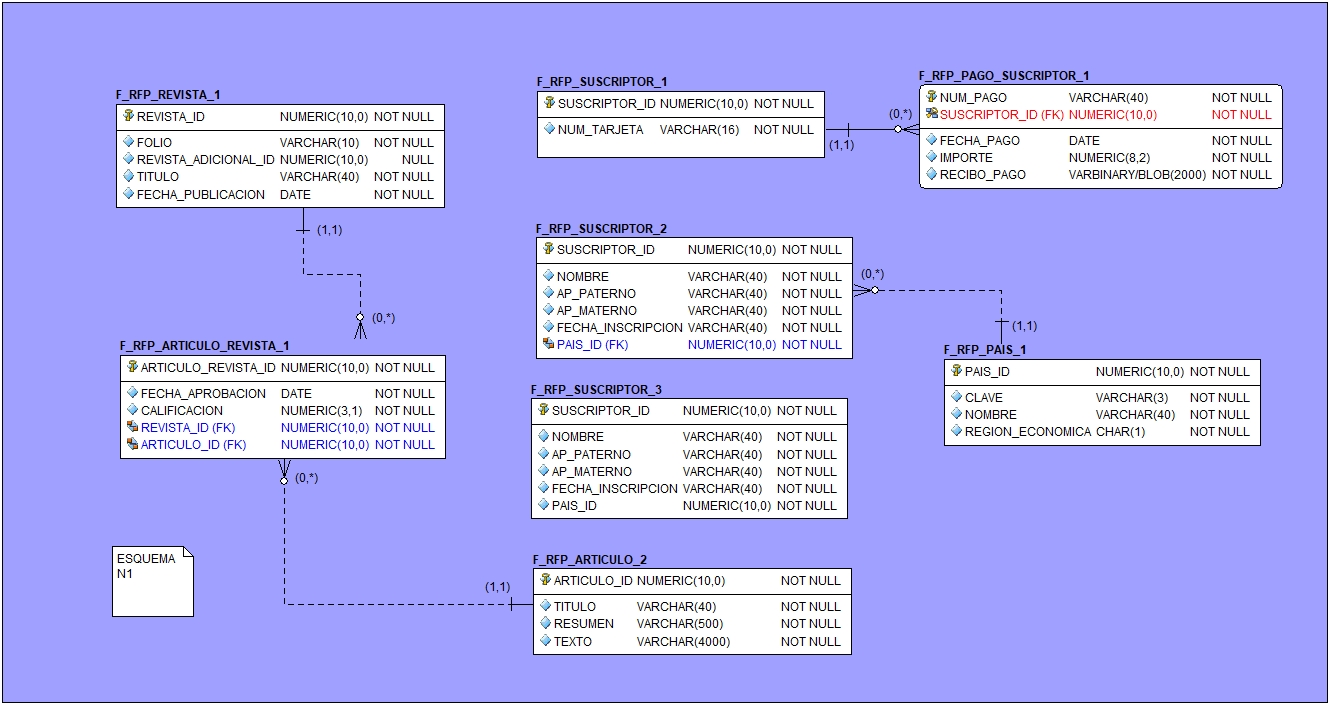
\includegraphics[width=\linewidth]{bdd_prac_04-n1.jpg}\\

% \newpage
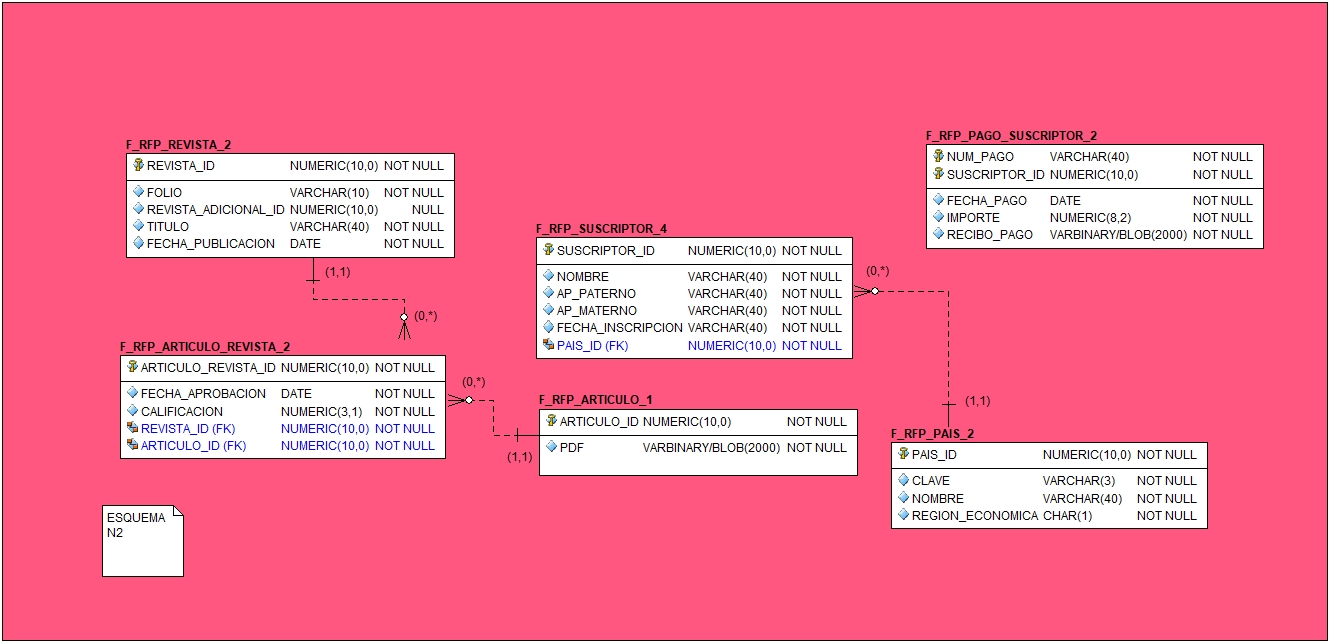
\includegraphics[width=\linewidth]{bdd_prac_04-n2.jpg}

\section*{Comentarios y conclusiones}

A pesar de solo contar con 2 nodos, esta práctica tuvo un cierto nivel de 
dificultad, realizar el proceso de fragmentación fue sencillo, pero a la hora
de construir los modelos relacionales se tuvo que tener especial cuidado con
las llaves foráneas, muchas de las FK se eliminaron, lo que provocó que varias 
tablas se quedarán ``aisladas'', es decir, que no se relacionarán con ninguna 
otra (aparentemente). Lo anterior fue nuevo y hasta llegue a pensar que estaba
mal, pero después de algo de análisis concluí que el modelo estaba bien, para
ello tuve que pensar en como se implementarían algunas sentencias DML.

\renewcommand\refname{Bibliografía}
\begin{thebibliography}{99}
    \bibitem{oracle} Oracle. \textit{Oracle Database Documentation} en 
        \texttt{https://docs.oracle.com/en/database/oracle/\\oracle-database/%
        index.html}
    %  TODO:- Add more references
\end{thebibliography}

\end{document}
